\documentclass[10pt]{article}
\usepackage[UTF8]{ctex}
\usepackage{picinpar,graphicx,bm}
\usepackage{booktabs}
\usepackage{diagbox}
\usepackage{float}
\usepackage{multirow}
\usepackage{textcomp}

\usepackage{listings}
\usepackage{xcolor}
% 定义可能使用到的颜色
\definecolor{CPPLight}  {HTML} {686868}
\definecolor{CPPSteel}  {HTML} {888888}
\definecolor{CPPDark}   {HTML} {262626}
\definecolor{CPPBlue}   {HTML} {4172A3}
\definecolor{CPPGreen}  {HTML} {487818}
\definecolor{CPPBrown}  {HTML} {A07040}
\definecolor{CPPRed}    {HTML} {AD4D3A}
\definecolor{CPPViolet} {HTML} {7040A0}
\definecolor{CPPGray}  {HTML} {B8B8B8}
\lstset{
    columns=fixed,    
   % numbers=left,                                        % 在左侧显示行号
    frame=none,                                          % 不显示背景边框
    backgroundcolor=\color[RGB]{245,245,244},            % 设定背景颜色
    keywordstyle=\color[RGB]{40,40,255},                 % 设定关键字颜色
    numberstyle=\footnotesize\color{darkgray},           % 设定行号格式
    commentstyle=\it\color[RGB]{0,96,96},                % 设置代码注释的格式
    stringstyle=\rmfamily\slshape\color[RGB]{128,0,0},   % 设置字符串格式
    showstringspaces=false,                              % 不显示字符串中的空格
    language=c++,                                        % 设置语言
    morekeywords={alignas,continute,friend,register,true,alignof,decltype,goto,
    reinterpret_cast,try,asm,defult,if,return,typedef,auto,delete,inline,short,
    typeid,bool,do,int,signed,typename,break,double,long,sizeof,union,case,
    dynamic_cast,mutable,static,unsigned,catch,else,namespace,static_assert,using,
    char,enum,new,static_cast,virtual,char16_t,char32_t,explict,noexcept,struct,
    void,export,nullptr,switch,volatile,class,extern,operator,template,wchar_t,
    const,false,private,this,while,constexpr,float,protected,thread_local,
    const_cast,for,public,throw,std,size_t,__global__,__device__,__host__},
    emph={map,set,multimap,multiset,unordered_map,unordered_set,
    unordered_multiset,unordered_multimap,vector,string,list,deque,
    array,stack,forwared_list,iostream,memory,shared_ptr,unique_ptr,
    random,bitset,ostream,istream,cout,cin,endl,move,default_random_engine,
    uniform_int_distribution,iterator,algorithm,functional,bing,numeric,},
    emphstyle=\color{CPPViolet}, 
    frame=shadowbox,
    basicstyle=\footnotesize\ttfamily,
    tabsize=4,
}

\newcommand{\tabincell}[2]{\begin{tabular}{@{}#1@{}}#2\end{tabular}}  
\newcommand{\upcite}[1]{\textsuperscript{\textsuperscript{\cite{#1}}}}

%layout
\usepackage{calc} 
\setlength\textwidth{7in} 
\setlength\textheight{9in} 
\setlength\oddsidemargin{(\paperwidth-\textwidth)/2 - 1in}
\setlength\topmargin{(\paperheight-\textheight -\headheight-\headsep-\footskip)/2 - 1.5in}


\title{基于多目视觉的人体测量系统}
\author{11821095 葛林林}
\begin{document}
\maketitle


\section{研究背景与意义}
随着现代科技的发展和生活水平的提高,人们对于产品的人性化需求也越来越高,因此产品的人性化设计成为设计高质量产品过程中需要重视的因素之一。人性化设计的产品能够增加舒适度和减少工伤数量。
\par 人体测量是对人体的尺寸、形状、长度以及工作能力进行测量,它是人体科学的一个重要的分支,其中人体外形的尺寸数据是人体测量中最重要的组成部分,可以用来作为产品工效学设计和空间布局设计的基本技术依据。人体测量的应用涵盖了与人相关的各个领域,如服装号型设计、建筑装修设计、家具设计、产品造型设计、机械制造、交通工具座舱设计、公共设施设计、医疗工程、人体仿真等。近年来,随着数字媒体产业的迅速发展,高精细的人体模型数据还在人机交互、虚拟现实、三维影视特效、三维游戏等中扮演着极为重要的角色。因此,人体测量技术得到了世界各国的高度重视和深入研究。

\section{国内外研究现状}
传统的人体尺寸数据库主要是采用人体测量尺测量得到。然而人工测量的方案存在主观性强、误差随机性大、效率低和可重复性差的缺点,并且测量结果缺乏完整的三维人体信息,其应用范围非常有限。近年来,随着各种三维扫描与测量设备的普及,人体测量逐渐从传统的尺寸测量向完整的三维人体外形扫描和测量发展\upcite{measurement01},并开始建立相应的三维人体模型数据库。与传统的人体测量尺寸相比,三维人体模型数据中所蕴涵的信息更为丰富,其应用领域和范围也更加宽广。
\par CAESAR产品系列(Civilian American and European Surface Anthropometry Resource)是国际上第一个大型三维人体测量项目。无论是设计新的服装系列还是驾驶舱,精确的车身尺寸对于创造更好,更具成本效益的产品至关重要。该产品系列汇集了来自服装,航空航天和汽车等众多行业的代表。CAESAR最初是政府和行业之间的合作伙伴关系,用于收集和组织最广泛的消费者身体测量样本以进行比较。该项目收集并组织了2,400名美国和加拿大以及2,000名欧洲平民的数据,并开发了一个数据库。随后,欧美和部分亚洲国家陆续开展了大量的关于人体测量的项目,例如德国Vitronic公司生产的VITUS全身3D人体扫描仪和体积更小的Vitus smart\upcite{measurement02}。我国目前的《中国成年人人体尺寸》标准建立于20年前。2005年,中国标准化研究院开始使用三维扫描仪对全国2万多个未成年进行了人体三维扫描,建立了中国未成年人三维人体模型数据库;2013年,中国标准化研究院开始使用三维扫描仪进行中国第二次成年人人体扫描和尺寸测量工作,准备建立中国成年人三维人体模型数据库。此外,国内研究人员和商业公司还陆续采用三维人体扫描仪开展过一些中小规模的三维人体测量项目,例如东华大学服装学院、北京服装学院、恒源祥集团等。
\par 目前,三维人体模型获取主要采用三维扫描仪或RGBD相机。三维扫描仪基于激光测距或结构光原理[3][4],其优势在于鲁棒性强、扫描分辨率高。最新的扫描仪其理论测量精度可达0.2mm,非常适合于静态刚体的外形获取,如机械零件、产品外形、静态文物等。但是,三维扫描仪的一个显著不足是测量时间较长。例如,目前成熟的三维扫描仪扫描整个人体最快也需要10秒左右。众所周知,人体是非刚体,即使是专业模特,也难以在长达数秒的扫描时间内保持姿势完全静止。正因如此,在人像摄影中,快门时间通常设定在数十分之一秒、百分之一秒内甚至更高以保证拍摄对象的清晰。因此,传统的三维人体扫描结果应为不同角度(获取方向)、不同时间(10秒内)和不同姿态(10秒或更长时间内小幅运动)的多个人体外形的混合,必然会存在原始数据误差、点云配准误差、表面重建误差等一系列误差,从而对最终获取的三维人体模型的精度产生较大影响。此外,由于需要相对较长的扫描时间,这种方式难以获得时空一致的人体表面纹理。RGBD相机是近年来出现并得到普及的三维信息获取和体感交互设备,代表性的设备是微软的Kinect[5]。由于集成了红外深度相机并采用硬件加速,Kinect具有实时性好、成本低廉的优点,并在面向游戏和数字娱乐的快速人体建模中得到应用[6]。然而,RGBD相机的获取分辨率低、数据的噪声大;此外,采用RGBD相机进行多角度的完整人体扫描,仍然需要至少3秒时间[7]。因此,重建的人体模型精度较低,尚不能满足高精度人体建模的需求。
\par 随着数字成像技术的快速发展,我们已经可以方便地获取千万像素级别甚至更高的数字照片。在这些照片中,人体表面的一些细节,如皮肤上的皱纹、凹凸、色斑、毛发等,可以表现得淋漓尽致。这提示我们在可控的漫射光环境下,如果实现多台相机在多个角度同步拍摄,那么我们就可以获得人体模型的瞬间投影,实现人体模型的“刚体”采集,避免传统扫描方法中存在的时间和姿态不同步的问题,并可以获得时空一致的表面纹理。这提示我们可以基于高分辨率照片、采用同步多双目立体视觉的方法实现高精度人体模型的重建[8][9]。
\par 但是,在大量高分辨率图像条件下,基于多双目立体视觉的高效、高精度和鲁棒三维重建仍然是一个具有挑战性的问题,仍然存在弱纹理匹配困难、点云恢复效率低、大量点云配准精度差、点云重构效率和精度不高等一系列难题。因此,基于同步多双目立体视觉的高精度人体建模的相关研究,不仅可以发展和完善立体视觉和数字几何处理中的相关理论和方法,高效地建立高精度人体模型;而且相关硬件和软件系统的研究和开发,可以形成一种全新的三维扫描系统原型,该系统可以在瞬间获取非刚体外形,克服传统三维扫描设备采集时间长、所获取的数据时空不一致的问题。此外,基于多双目立体视觉的高精度人体建模的研究,还是构建高精度人体模型数据库的基础和关键技术,不仅在服装、建筑、家居、制造、交通等重要领域有着广泛应用,同时在医疗工程、人体仿真、人机交互、虚拟现实、三维影视动画、三维游戏等产业中扮演着极为重要的角色。

\section{基于多目的三维重建系统简介}
基于多目的三维重建系统是以Multi-View Stereo (MVS)理论为基础对人体进行重建。该系统中包含81架单反相机,由于在整个人体模型当中人脸部分较为复杂,因此在这些相机当中有6架高分辨相机专门拍摄人脸照片,从而获得更多的人脸信息。基于多目的三维重建系统的具体处理流程图如下图所示:
\begin{figure}[H]
\begin{center}
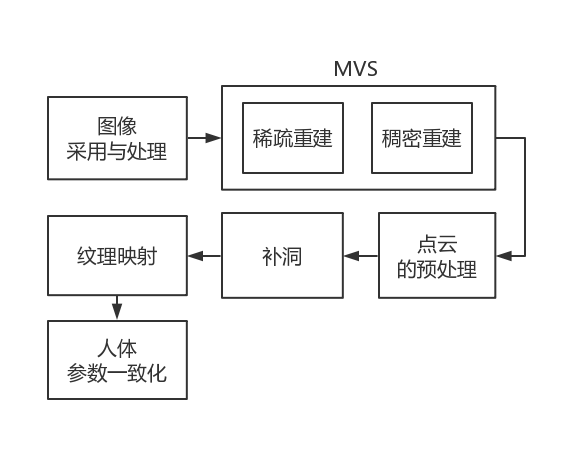
\includegraphics[scale=0.5]{schematic.png}
\caption{基于多目的三维重建系统流程示意图}
\end{center}
\end{figure}
\section{图像采集与预处理}
当获取到人体图片之后,需要进行图片的预处理,首先要将背景从图片中剔除掉,从而得到干净的人体点云数据。本课题中利用深度学习的方法实现了批量化的图像自动化前景背景分割。如下图所示是利用既有深度学习的自动化前景背景分割得到的效果图。
\begin{figure}[H]
\begin{center}
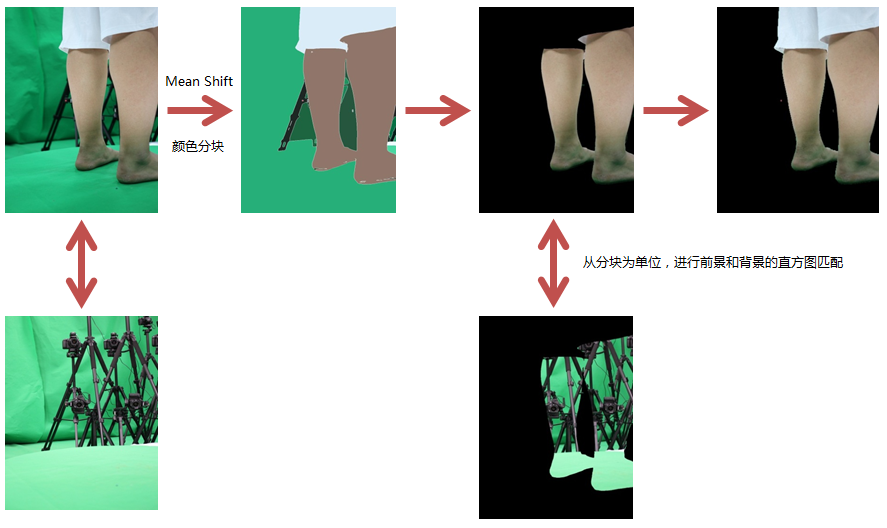
\includegraphics[scale=0.3]{image_pre_processing.png}
\caption{人体图片创建mask示意图}
\end{center}
\end{figure}

\section{Multi-View Stereo (MVS)}
\subsection{稀疏重建}
稀疏重建的目的是根据图像特征点之间的匹配关系从而估算出相机的内外参信息,这个过程又被称为Structure From Motion (SFM)。它是将3D结构从其投影重建为一系列图像的过程。 输入是从不同视点获取的同一对象的一组重叠图像。 输出是对象的3-D重建,以及所有图像的重建的内在和外在相机参数。SFM大体可以分为两种方案:
\begin{itemize}
\item{增量式SFM}
\begin{itemize}
\item{首先,根据两个相机图片之间的匹配点集计算出两个相机的位姿;}
\item{随后在添加一个相机进行位姿的解算;}
\item{并且利用Bundle Adjustment算法对相机位姿进行优化;}
\item{添加新相机,重复上述第二步开始的过程。}
\end{itemize}


\item{全局SFM}
\begin{itemize}
\item{首先,根据图片集估计相机之间的Fundamental Matrix;}
\item{建立图结构;}
\item{对图结构进行优化;}
\item{对所有相机计算Bundle Adjustment。}
\end{itemize}
\end{itemize}
本系统中采用了增量式SFM方案,一般该方案的处理过程可以分为如下三个阶段:
\begin{itemize}
\item{特征检测和提取}
\item{特征匹配和几何验证}
\item{结构和运动重建}
\end{itemize}
\subsubsection{图像特征提取和匹配}
在多目重建中为了计算相机的内外参数必须先提取出图像中的特征点,本系统中使用的sift特征,根据sift特征在在相邻的视图中寻找匹配点,再根据得到的匹配点信息通过八点算法等计算出两个相机之间的基本矩阵。
\subsubsection{内外参的计算}
内外参的计算主要体现在Bundle Adjustment算法上,Bundle Adjustment算法主要是求取如下目标函数的一个算法,该该目标函数也被称为重投影误差:
\begin{equation}
E(P,M)=\sum_j \sum_{i \in V(j)} |P_i(M^j)-m_i^j|^2
\end{equation}
其中,${P_i}$代表的是一些相机参数,$M^j$代表三维点位置,$m_i^j$代表的是三维点$M^j$对应在第i个相机上的图像坐标系下的坐标点。一般利用Levenberg-Marquardt算法来计算该目标函数。

\subsection{稠密重建}
Multi-View Stereo(MVS)是生成密集点云的方法,由于SFM是根据特征点得到的稀疏点云,根据特征点无法得到稠密的三维点云,而MVS则几乎对照片中的每个像素点都进行匹配,几乎重建每一个像素点的三维坐标,这样得到的点的密集程度可以较接近图像为我们展示出的清晰度。其实依据的理论在于多视图照片间拍摄到的相同的三维几何结构部分存在极线几何约束。
\subsubsection{图像畸变矫正(Undistorsion)}
由于相机工业的原因不可避免的存在相机的畸变,因此需要利用相机畸变模型对图像进行矫正,畸变分为径向畸变和切向畸变。
\subsubsection{块匹配(Patch Match)}
在对极约束的基础上,接下来就是在图片上的一条线上进行探测,寻找两张图片上的同一点。主要方法为逐像素判断,两个照片上的点是否是同一点,为此提出图像点间的“一致性判定函数”如下所示。
\begin{equation}
C_{ij}(p)=\rho(I_i(\Omega(\pi_i(p))),I_j(\Omega(\pi_j(p))))
\end{equation}
其中$\pi(p)$是使得点p投影到照片上一点的函数,$\Omega(x)$函数定义了一个点$x$周围的区域,$I(x)$函数代表了照片区域的强度特征,$\rho(f,g)$是用来比较两个向量之间的相似程度的。$\rho$函数和$\Omega$函数的具体选择决定这个”一致性判别“的准确度。

\subsubsection{立体融合(Stereo Fusion)}
\subsubsection{泊松重建(Poisson Mesher)}

\section{点云数据的预处理}
点云的预处理有法向估计、去噪、重采样等,点云的法向在去噪、重采样等操作中拥有很重要的作用,因此首先要进行点云法向的估计,如下图所示是得到的点云法向估计的效果图。
\begin{figure}[H]
\begin{center}
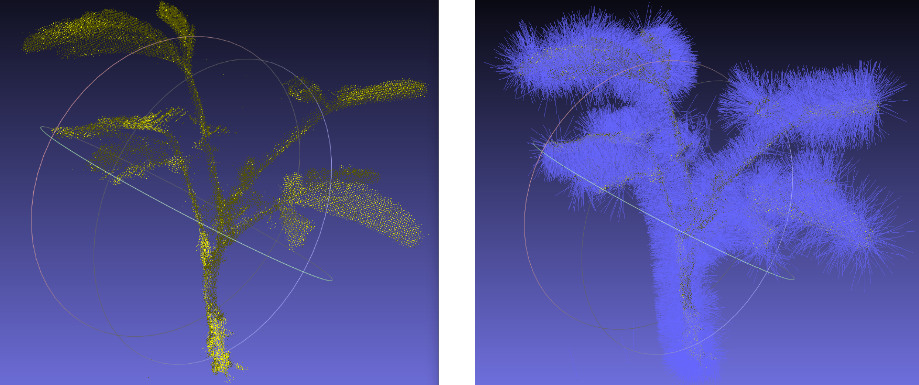
\includegraphics[scale=0.3]{normal-estimation.png}
\caption{基于双目的三维重建系统流程示意图}
\end{center}
\end{figure}
关于点云去噪的方法有很多,大致分为如下几类:(1)基于MLS的滤波方法;(2)基于粒子的去噪方法\upcite{filter01}$^{^{-}}$\upcite{filter05};(3)基于稀疏理论的方法\upcite{filter06}$^{^{-}}$\upcite{filter10}。然而并没有很好的方法能够同时应对离群点的处理以及点云表面平滑的处理。因此本课题在进行点云的去噪将离群点的剔除以及点云表面的平滑处理作为两个步骤分别进行处理。针对点云的去噪处理能够有效的减小后期点云处理的误差,使得后期的点云处理操作更加鲁棒,如下图所示是利用一些点云处理算法得到的点云滤波结果图。
\begin{figure}[H]
\begin{center}
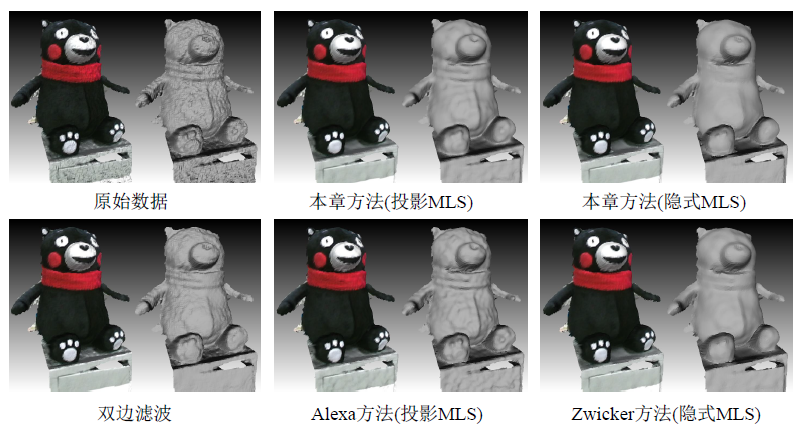
\includegraphics[scale=0.3]{point-cloud-denoising.png}
\caption{基于双目的三维重建系统流程示意图}
\end{center}
\end{figure}
由于点云数据量十分庞大,如果利用原始的点云数据进行刚性配准,则配准的过程将十分缓慢,因此在进行下一步的刚性配准之前需要进行点云的重采样。如下图所示是基于C-WLOP方法得到的点云重采样效果的示意图。
\begin{figure}[H]
\begin{center}
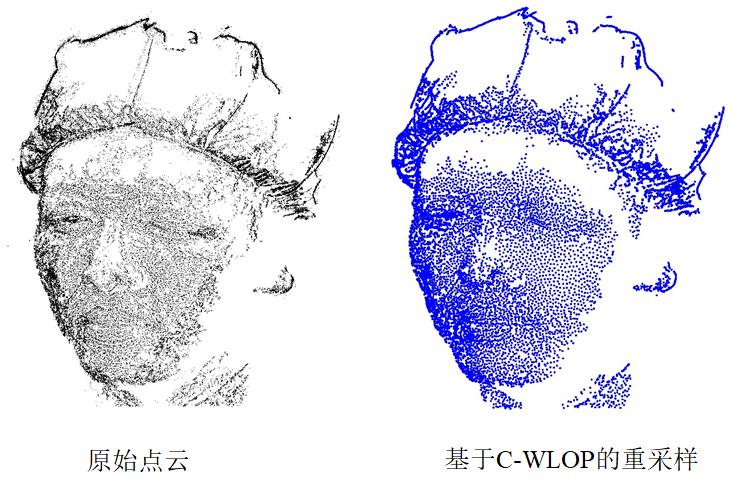
\includegraphics[scale=0.25]{point-cloud-resampling.png}
\caption{基于双目的三维重建系统流程示意图}
\end{center}
\end{figure}

\section{补洞}
非结构化的点云数据通常不便于直接进行处理,一些学者将其嵌入到空间体网格之中,在此基础上寻找对应缺失区域的体网格,并产生新的数据点对其进行合理填充,这是基于体的孔洞修补方法的基本思想。
\section{纹理映射}
纹理映射是在不增加几何表面复杂度的基础上,有效地还原展现三维模型的表面细节特征,进而提高物体的真实感\upcite{texture_mapping01}。如下图所示是补洞前后的效果图:
\begin{figure}[H]
\begin{center}
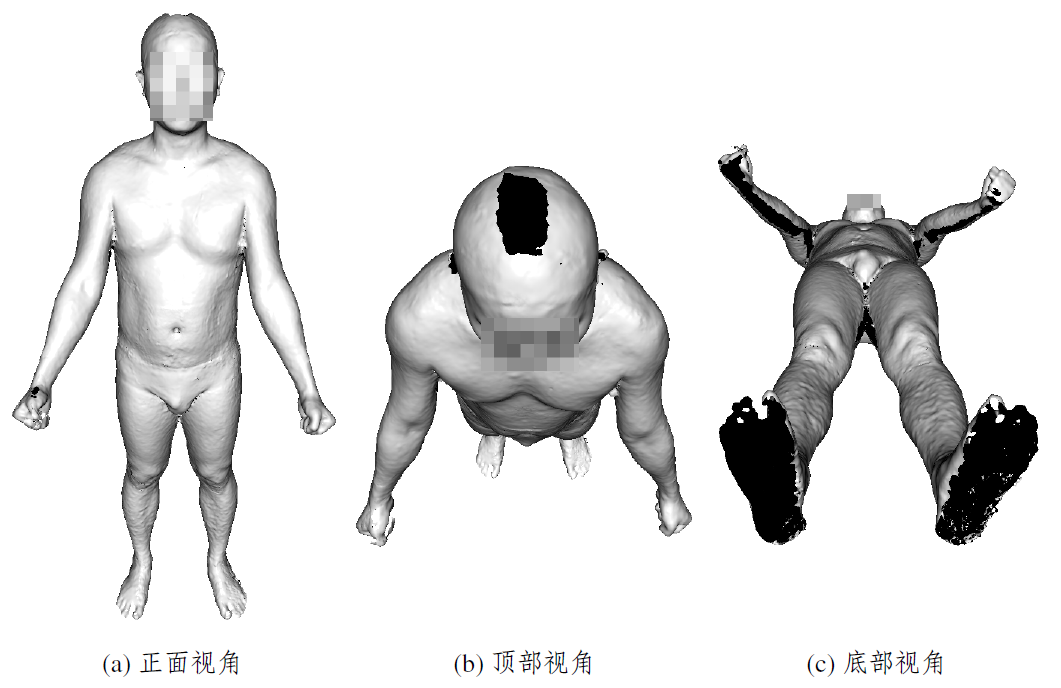
\includegraphics[scale=0.25]{filling-hole.png}
\caption{基于双目的三维重建系统流程示意图}
\end{center}
\end{figure}

\begin{figure}[H]
\begin{center}
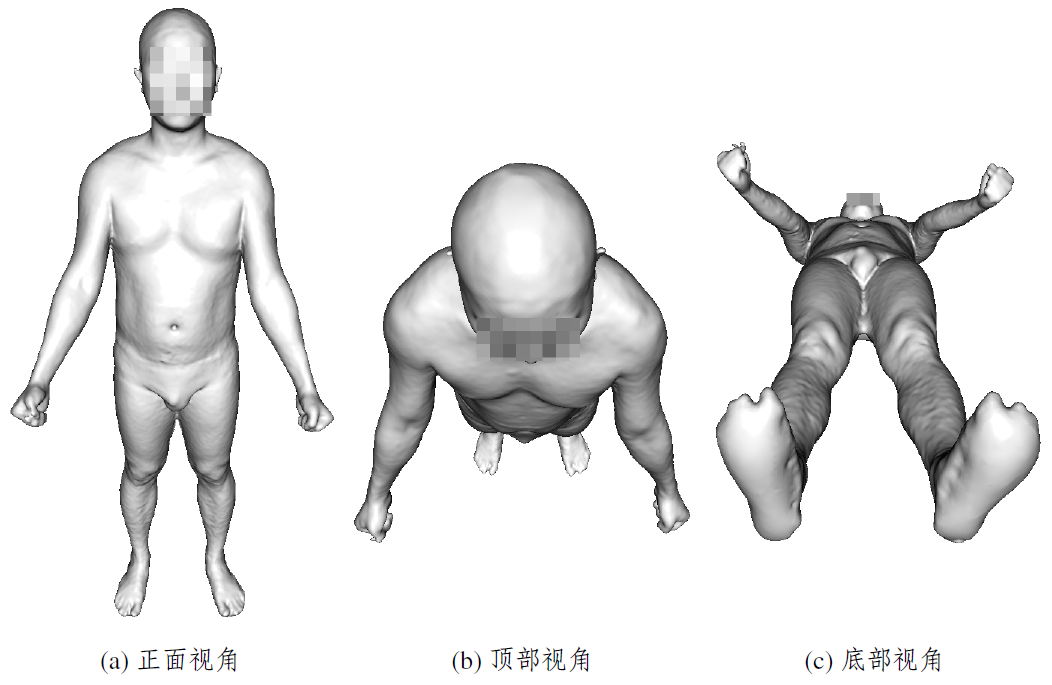
\includegraphics[scale=0.25]{filling-hole-effect.png}
\caption{基于双目的三维重建系统流程示意图}
\end{center}
\end{figure}

\section{人体参数一致化}
人体参数一致化的步骤分为人体模型骨架提取、非等距模型之间对应关系求解和模型的一致参数化。人体模型骨架的提取是提供模型块对应关系,同时区分出人体的左右对称。非等距模型之间对应关系的求解是为了建立不同人体模型之间点与点之间的对应关系。模型的一致参数化是为了使得模型具有相同的顶点和一致的连接关系。如下图所示是参数一致化过程中的部分结果。
\begin{figure}[H]
\begin{center}
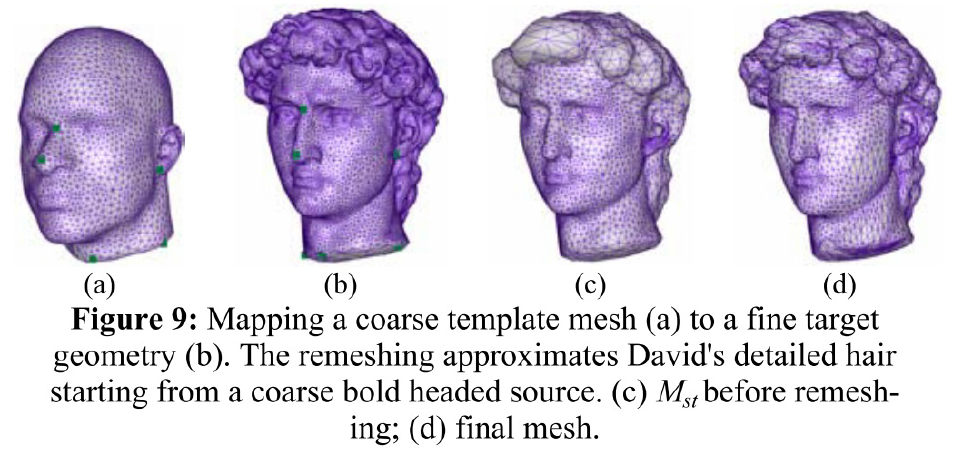
\includegraphics[scale=0.3]{parameter.png}
\caption{基于双目的三维重建系统流程示意图}
\end{center}
\end{figure}


\section{未来展望}
本文主要介绍了利用双目视觉的方法进行三维重建,然而基于双目视觉的方法存在许多弊端,例如标定过程非常繁琐和耗时,双目结构一旦发生移动就需要重新标定,一旦系统某个相机缺失图片就会导致某个视角的点云缺失等。基于多目视觉的重建技术能够很好的克服上述问题。双目视觉由于利用了自标定技术不需要手动的进行相机内参的标定,并且由Bundle Adjust算法能够较为精准的算出相机的外参。除此之外,由于多目系统存在很多的重叠区域,因此一旦某个相机停止工作,并不会影响到整个人体的重建。所以基于多目的重建系统将是接下来的研究重点。
\par 除此之外,人体测量技术的应用十分广泛,因此可以开展针对于人体测量技术应用方面的研究。首先可以建立具有不同性别、年龄、身高、体态等分布人体模型库,其具体目标如下所示:(1)要求人体模型数据库的测量精度能够达到2mm;(2)要求人体模型数据库可以用网格、细分曲面、NURBS曲面、隐式曲面等表示;(3)要求人体模型数据库拥有低分辨率、中等分辨率、高精细三个版本。其次可以开发一套基于人体测量技术的快速试衣系统,该系统能够根据自身的人体模型给出衣服合身与否的结论,从而帮助人们在线的选择合身的衣服。


\begin{thebibliography}{1}
\bibitem{measurement01} 张文斌, 肖平, 杨子田,等. 人体测量高新技术——三维人体扫描技术的应用和发展[C] 2006/2007中国纺织工业技术进步研究报告. 2006.
\bibitem{measurement02} 罗仕鉴, 朱上上, 孙守迁. 人体测量技术的现状与发展趋势[J]. 人类工效学, 2002, 8(2):31-34.
\bibitem{measurement03} Anguelov, D., Srinivasan, P., Koller, D., et al. Scape: Shape Completion and Animation of People. ACM Transactions on Graphics (TOG), 2005, 24(3): 408–416.
\bibitem{measurement04}[4]	Hasler, N., Stoll, C., Sunkel, M., et al. P. A statistical model of human pose and body shape. Computer Graphics Forum, 2009, 28(2): 337-346.
\bibitem{measurement05}	Newcombe, R. A., Davison, A. J., Izadi, S., et al. KinectFusion: Real-time dense surface mapping and tracking. Proceedings of IEEE 10th International Symposium on Mixed and Augmented Reality (ISMAR), 2011, 127–136.
\bibitem{measurement06}	Tong, J., Zhou, J., Liu, L., Pan, Z., and Yan, H. Yan. Scanning 3D Full Human Bodies Using Kinects. IEEE Transactions on Visualization and Computer Graphics (TVCG), 2012, 18(4): 643–650.
\bibitem{measurement07}	Chen, Y., Dang, G., Cheng, Z. Q., et al. Fast capture of personalized avatar using two Kinects. Journal of Manufacturing Systems, 2014, 33(1): 233-240.
\bibitem{measurement08}	Seitz, S. M., Curless, B., Diebel, J., Scharstein, D., and Szeliski, R. A comparison and evaluation of multiview stereo reconstruction algorithms. Proceedings of IEEE CVPR, 2006, 1: 519–528.
\bibitem{measurement09}	Starck, J., and Hilton, A. Surface capture for performance based animation. IEEE Computer Graphics and Applications, 2007, 27(3): 21–31.
\bibitem{measurement10}	Dong, Q., Feng, J. (2019). Outlier detection and disparity refinement in stereo matching. Journal of Visual Communication and Image Representation.
\bibitem{measurement11}	Dong, Q., Feng, J. (2018). Adaptive disparity computation using local and non-local cost aggregations. Multimedia Tools and Applications, 77(24), 31647-31663.
\bibitem{filter01}	Lipman, Y., Cohen-Or, D., Levin, D.,  Tal-Ezer, H. (2007, August). Parameterization-free projection for geometry reconstruction. In ACM Transactions on Graphics (TOG) (Vol. 26, No. 3, p. 22). ACM.
\bibitem{filter02}	Huang, H., Li, D., Zhang, H., Ascher, U., Cohen-Or, D. (2009). Consolidation of unorganized point clouds for surface reconstruction. ACM transactions on graphics (TOG), 28(5), 176.
\bibitem{filter03}	Huang, H., Wu, S., Gong, M., Cohen-Or, D., Ascher, U.,  Zhang, H. R. (2013). Edge-aware point set resampling. ACM transactions on graphics (TOG), 32(1), 9.
\bibitem{filter04}	Preiner, R., Mattausch, O., Arikan, M., Pajarola, R.,  Wimmer, M. (2014). Continuous projection for fast L1 reconstruction. ACM Trans. Graph., 33(4), 47-1.
\bibitem{filter05}	Liao, B., Xiao, C., Jin, L.,  Fu, H. (2013). Efficient feature-preserving local projection operator for geometry reconstruction. Computer-Aided Design, 45(5), 861-874.
\bibitem{filter06}	Avron, H., Sharf, A., Greif, C.,  Cohen-Or, D. (2010). ℓ 1-Sparse reconstruction of sharp point set surfaces. ACM Transactions on Graphics (TOG), 29(5), 135.
\bibitem{filter07}	Xiong, S., Zhang, J., Zheng, J., Cai, J.,  Liu, L. (2014). Robust surface reconstruction via dictionary learning. ACM Transactions on Graphics (TOG), 33(6), 201.
\bibitem{filter08}	Mattei, E.,  Castrodad, A. (2017, December). Point cloud denoising via moving rpca. In Computer Graphics Forum (Vol. 36, No. 8, pp. 123-137).
\bibitem{filter9}	Sun, Y., Schaefer, S.,  Wang, W. (2015). Denoising point sets via L0 minimization. Computer Aided Geometric Design, 35, 2-15.
\bibitem{filter10}	Xu, L., Wang, R., Zhang, J., Yang, Z., Deng, J., Chen, F.,  Liu, L. (2015). Survey on sparsity in geometric modeling and processing. Graphical Models, 82, 160-180.
\bibitem{non_rigid_register01}	唐逸之, 罗闪, 冉清,等. 基于多薄板样条的多视角非刚性配准算法[J]. 计算机辅助设计与图形学学报, 2017, 29(12):2153-2161.
\bibitem{texture_mapping01}	朱礼楠. 面向多视图三维重建的纹理映射方法[D]. 2018.
\end{thebibliography}

\end{document}